

Most problems in machine learning require minimization/maximization of functions (likelihoods, risk, energy, entropy, etc.,). Let $x^*$ be the value of $x$ which minimizes the value of some function $f(x)$. Mathematically, this is written as

\begin{equation*}
x^* = \argmin_x f(x)
\end{equation*}

In a few special cases, we can solve this minimization problem analytically in closed form (solving for optimal $x^{*}$ in  $\nabla_{x}f(x^{*})=0$), 
but in most cases it is too cumbersome (or impossible) to solve these equations analytically, and they must be tackled numerically. In this section we will cover some basic notions of numerical optimization. The goal is to provide the intuitions behind the methods that will be used in the rest of the school. There are plenty of good textbooks in the subject that you can consult for more information \citep{Nocedal1999,bertsekas1995np,boyd2004convex}.

The most common way to solve the problems when no closed form solution is available is to resort to an iterative algorithm. In this Section, we will see some 
of these iterative optimization techniques. These iterative algorithms compute a sequence of points $x^{(0)},x^{(1)},\ldots \in \text{domain}(f)$ such that hopefully $x^t = x^*$.
Such a sequence is called the {\bf minimizing sequence} for the problem.


\subsection{Convex Functions}

One important property of a function $f(x)$ is whether it is a \textbf{convex function} (in the shape of a bowl) or a \textbf{non-convex function}. Figures \ref{fig:convexfn} and \ref{fig:nonconvexfn} show an example of a convex and a non-convex function. Convex functions are particularly useful since you can guarantee that the minimizing sequence converges to the true global minimum of the function, while in non-convex functions you can only guarantee that it will reach a local minimum. 


 \begin{figure}[h]
 \begin{center}
     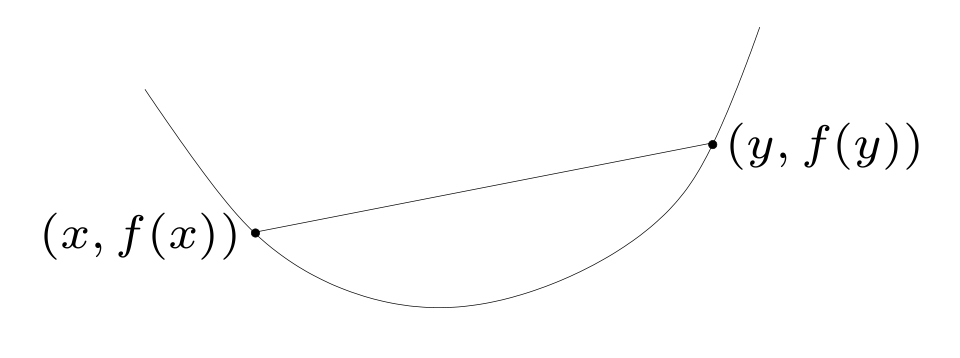
\includegraphics[width=0.6\columnwidth]{figs/intro/convexfn.png}
   \caption{\label{fig:convexfn} Illustration of a convex function. The line segment between any two points on the graph lies entirely above the curve.} 
     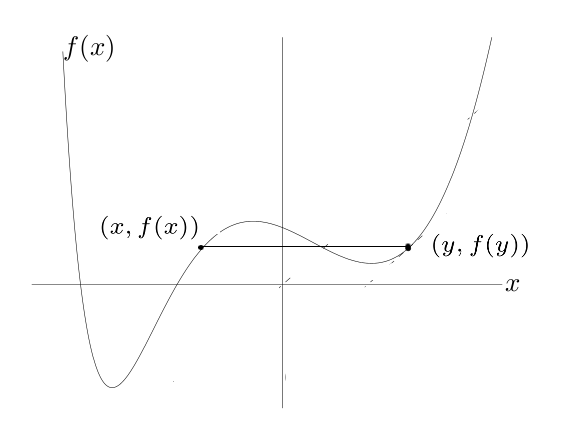
\includegraphics[width=0.5\columnwidth]{figs/intro/nonconvexfn.png}
   \caption{\label{fig:nonconvexfn} Illustration of a non-convex function. Note the line segment intersecting the curve. } 
 \end{center}
 \end{figure}


Intuitively, imagine dropping a ball on either side of 
Figure
\ref{fig:convexfn}, the ball will role to the bottom of the bowl
independently from where it is dropped. This is the main benefit of a
convex function. On the other hand, if you drop a ball from the left
side of Figure \ref{fig:nonconvexfn} it will reach a
different position than if you drop a ball from its right side. Moreover, dropping it from the left side will lead you to a much better (\emph{i.e.}, lower) place than if you drop the ball from the right side. This is the main problem with non-convex functions: there are no guarantees about the quality of the local minimum you find.

More formally, some concepts to understand about convex functions are:

A {\bf line segment} between points $x_{1}$ and $x_{2}$: contains all points such that 
\begin{equation*}
x=\theta x_{1} + (1-\theta)x_{2}
\end{equation*}
where $0\leq \theta \leq 1$.

\vspace{0.1in}
A {\bf convex set} contains the line segment between any two points in the set 
\begin{equation*}
x_{1}, x_{2} \in C,\hspace{0.12in} 0 \leq \theta \leq 1 \hspace{0.12in} \Rightarrow \hspace{0.12in} \theta x_{1} + (1-\theta)x_{2} \in C
\end{equation*}

\vspace{0.1in}
A function $f: \mathbb{R}^{n}\rightarrow R$ is a {\bf convex function} if the domain of $f$ is a convex set and 
\begin{equation*}
f(\theta x + (1-\theta) y) \leq \theta f(x) + (1-\theta) f(y)
\end{equation*}

for all $x,y \in \text{domain of } f$, $0 \leq \theta \leq 1$

\subsection{Derivative and Gradient}

The \textbf{derivative} of a function is a measure of how the function varies with its input variables. 
Given an interval $[a,b]$ one can compute how the function varies within that interval by calculating the average slope of the function in that interval. 
\begin{equation}
\frac{f(b) - f(a)}{b-a} 
\end{equation}
The derivative can be seen as the limit as the interval goes to zero, and it gives us the slope of the function at that point.
\begin{equation}
\frac {\partial f}{\partial x} = \lim_{h = 0} \frac{f(x+h) - f(x)}{h} 
\end{equation}

Table \ref{tb::derivatives} shows derivatives of some functions that we will be using during the school. 

\begin{table}
\begin{center}
\begin{tabular}{|l|l|}
\hline
Function $f(x)$& Derivative $\frac{\partial f}{\partial x}$\\
\hline
$x^2$ & $2x$\\
\hline
$x^n$ & $nx^{n-1}$\\
\hline
$\log(x)$ & $\frac{1}{x}$\\
\hline
$\exp(x)$ & $\exp(x)$\\
\hline
$\frac{1}{x}$ & $-\frac{1}{x^{2}}$\\
\hline
\end{tabular}
\end{center}
\caption{\label{tb::derivatives}Some derivative examples}
\end{table}

An important rule of derivation is the chain rule. Consider $h=f\circ g$, and $u=g(x)$, then:

\begin{equation}
\frac{\partial h}{\partial x}=\frac{\partial f}{\partial u}\cdot\frac{\partial g}{\partial x}
\end{equation}

\begin{example}


Consider the function $h(x)=exp(x^{2})$. \\
$h(x)=f(g(x))=f(u)=exp(u)$, where $u=g(x)=x^{2}$.\\
$\frac{\partial h}{\partial x}=\frac{\partial f}{\partial u}\cdot \frac{\partial u}{\partial x}=exp(u) \cdot 2x=exp(x^{2}) \cdot 2x$\\

\end{example}

\begin{example}
Consider the function $f(x) = x^2$ and its derivative $\frac{\partial f} {\partial x}$. Look at the derivative of that function at points [-2,0,2], draw the tangent to the graph in that point.

$\frac{\partial f}{\partial x}\left(-2\right)=-4$, $\frac{\partial f}{\partial x}\left(0\right)=0$, and $\frac{\partial f}{\partial x}\left(2\right)=4$

For example, the tangent equation for $x=-2$ is $y=-4x - b$, where $b=f(-2)$

The following code plots the function and the derivatives on those
points using matplotlib (See Figure \ref{fig:tangents}).
\begin{python}
a = np.arange(-5,5,0.01)
f_x = np.power(a,2)
plt.plot(a,f_x)

plt.xlim(-5,5)
plt.ylim(-5,15)

k= np.array([-2,0,2])
plt.plot(k,k**2,"bo")
for i in k:
    plt.plot(a, (2*i)*a - (i**2))

\end{python}

\begin{figure}[h]
\begin{center}
   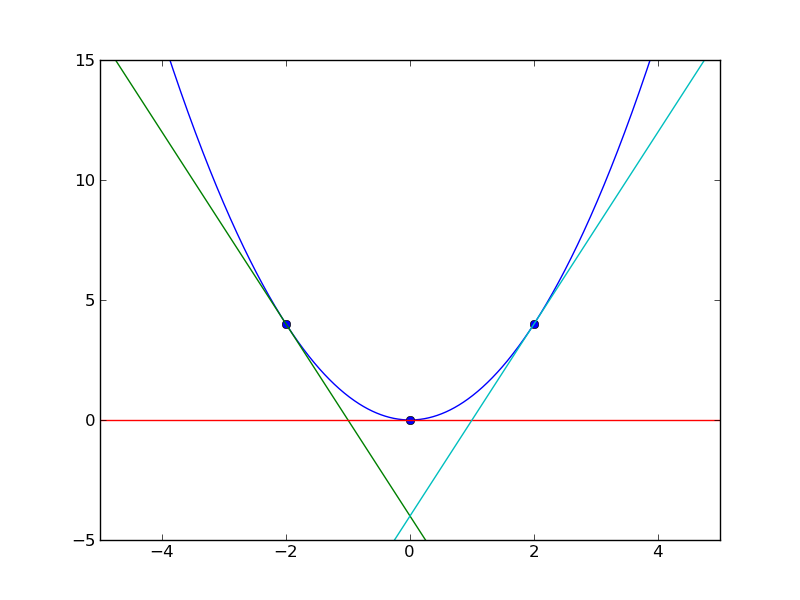
\includegraphics[width=0.6\columnwidth]{figs/intro/tangents.png}
 \caption{\label{fig:tangents} Illustration of the gradient of the
   function $f(x^2)$ at three different points $x = [-2,0.2]$. Note
   that at point $x = 0$ the gradient is zero which corresponds to the
 minimum of the function.}
\end{center}
\end{figure}


\end{example}

The \textbf{gradient} of a function is a generalization of the 
derivative concept we just saw before, for several dimensions. Lets
assume we have a function  $f(x)$ where $x \in \mathbb{R}^2$, so $x$ can be seen as
a pair $x = {x_1,x_2}$. Then, the gradient measures the slope of the
function in both directions: $\nabla_{x} f(x) = [\frac {\partial f}{\partial x_1},\frac {\partial f}{\partial x_2}]$.


\subsection{Gradient Based Methods}

Gradient based methods are probably the most common methods used for finding the minimizing sequence for a given function. The methods used in this class 
will make use of the function value $f(x)$ as well as the gradient of the function $\nabla_{x} f(x)$. 
The simplest method is the {\bf Gradient descent} method, an unconstrained first-order optimization algorithm. 

The intuition of this method is as follows: You start at a given point
$x_0$ and compute the gradient at that point $\nabla_{x_0} f(x)$. You
then take a step of length $\eta$ on the direction of the negative
gradient to find a new point: $x_1$ = $x_0 - \eta \nabla_{x_{0}}
f(x)$. Then, you compute the gradient at this new point, $\nabla_{x_1} f(x)$, and take a step of length $\eta$ on the direction of the negative
gradient to find a new point: $x_2$ = $x_1 - \eta \nabla_{x_{1}} f(x)$. You proceed until you have reached a minimum (local or global). Recall from the previous subsection that you can identify the minimum by testing if the norm of the gradient is zero: $||\nabla f(x)|| = 0$.

There are several practical concerns even with this basic algorithm to ensure both that the algorithm converges (reaches the minimum) and that it does so in a fast way (by fast we mean the number of function and gradient evaluations). 
\begin{itemize}
\item \textbf{Step Size $\eta$} A first question is how to find the step length $\eta$. One condition is that $eta$ should guarantee sufficient decrease in the function value. We will not cover these methods here but the most common ones are \textbf{Backtracking line search} or the \textbf{Wolf Line Search} \citep{Nocedal1999}.
\item \textbf{Descent Direction}  A second problem is that using the negative gradient as direction can lead to a very slow convergence. Different methods that change the descent direction by multiplying the gradient by a matrix $\beta$ have been proposed that guarantee a faster convergence. Two notable methods are the Conjugate Gradient (CG) and the Limited Memory Quasi Newton methods (LBFGS) \citep{Nocedal1999}. 
\item \textbf{Stopping Criteria} Finally, it will normally not be possible to reach full convergence either because it will be too slow, or because of numerical issues (computers cannot perform exact arithmetic). So normally we need to define a stopping criteria for the algorithm. Three common criteria (that are normally used together) are: a maximum number of iterations; the gradient norm be smaller than a given threshold   $||\nabla f(x)|| \leq \eta_1$, or the normalized difference in the function value be smaller than a given threshold $\frac{|f(x_t) - f(x_{t-1})|}{\max(|f(x_t)|,|f(x_{t-1})|)} \leq \eta_2$
\end{itemize}

Algorithm \ref{alg:graddescent} shows the general gradient based algorithm. Note that for the simple gradient descent algorithm $\beta$ is the identity matrix and the descent direction is just the negative gradient of the function, $\beta = -\nabla f(x)$. Figure \ref{fig:graddescent} shows an illustration of the gradient descent algorithm.

\begin{algorithm}[h]
\caption{Gradient Descent\label{alg:graddescent}}
\begin{algorithmic}[1]
\STATE {\bf given} a starting point $x_{0}, i=0$
\STATE {\bf repeat}
\STATE \quad Compute step size $\eta$
\STATE \quad Compute descent direction $- \beta\nabla f(x_{i})$.
\STATE \quad $x_{i+1} \leftarrow x_{i} - \eta\beta\nabla f(x_{i})$
\STATE \quad $i \leftarrow i + 1$
\STATE {\bf until} stopping criterion is satisfied.
\end{algorithmic}
\end{algorithm}

\begin{figure}[h]
\begin{center}
   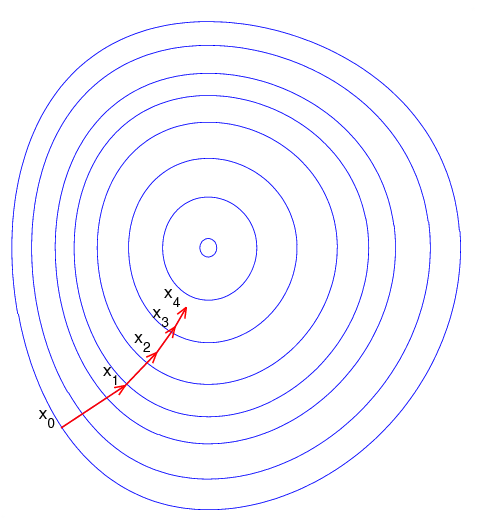
\includegraphics[width=0.6\columnwidth]{figs/intro/graddescent.png}
 \caption{\label{fig:graddescent} Illustration of gradient descent. The blue circles correspond to contours of the function (each blue circle is a set of points which have the same function value), while the red lines correspond to steps taken in the negative gradient direction.}
\end{center}
\end{figure}


% Gradient descent can work in any number of dimensions.  The process can also include {\bf line search} 
% to determine the locally optimal $\eta$ in each iteration. For non-differentiable functions, gradient 
% methods are ill-defined. Also, the procedure can take many iterations to converge to a local minimum 
% and methods based on Newton's method can be better alternatives. The main idea behind
% the iterative minimization techniques is find the locally best direction to move towards the (unknown) minimum. 
% While gradient descent moves in the direction of the negative gradient, other techniques like steepest 
% descent, conjugate descent, (L-)BGFS etc use other directions for update.

\begin{exercise}
Consider the function $f(x) = (x+2)^2 - 16 \exp\left( -(x-2)^2 \right)$.
Make a function that computes the function value given $x$.

\begin{python}
def get_y(x):
    value =  pow((x+2),2) - 16*math.exp(-((x-2)**2))
    return value
\end{python}

Draw a plot around $x \in [-8,8]$.

\begin{python}
x = np.arange(-8,8,0.001)
y = map(lambda u: get_y(u),x)
plt.plot(x,y)
plt.show()
\end{python}

Calculate the derivative of the function $f(x)$, implement the function \emph{get\_grad(x)}.

\begin{python}
def get_grad(x):
    return (2*x+4)-16*(-2*x + 4)*np.exp(-((x-2)**2))
\end{python}

Use the method \emph{gradient\_descent} to find the minimum of this function. Convince yourself that the code is doing the proper thing. Look at the constants we defined. Note, that we are using a simple approach to pick the step size (always have the value step\_size) which is not necessarily correct. 

\begin{python}
def gradient_descent(start_x,func,grad):
    # Precision of the solution
    prec = 0.0001
    #Use a fixed small step size
    step_size = 0.1
    #max iterations
    max_iter = 100
    x_new = start_x
    res = []
    for i in xrange(max_iter):
        x_old = x_new
        #Use beta egual to -1 for gradient descent 
        x_new = x_old - step_size * get_grad(x_new)
        f_x_new = get_y(x_new)
        f_x_old = get_y(x_old)
        res.append([x_new,f_x_new])
        if(abs(f_x_new - f_x_old) < prec):
            print "change in function values too small, leaving"
            return np.array(res)
    print "exceeded maximum number of iterations, leaving"
    return np.array(res)
\end{python}

Run the gradient descent algorithm starting from $x_0 = -8$ and plot the minimizing sequence.

\begin{python}
x_0 = -8
res = gradient_descent(x_0,get_y,get_grad)
plt.plot(res[:,0],res[:,1],'+')
plt.show()
\end{python}


\begin{figure}[h]
\begin{center}
   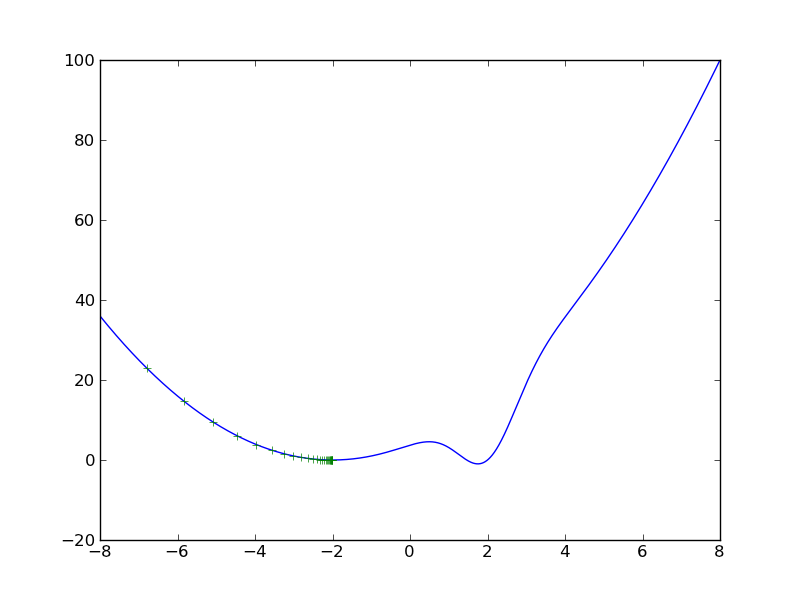
\includegraphics[width=1\columnwidth]{figs/intro/gradex1.png}
 \caption{\label{fig:gradex1} Example of running gradient descent
   starting on point $x_0 = -8$ for function $f(x) = (x+2)^2 - 16
   \exp\left( -(x-2)^2 \right)$. The function is represented in blue,
   while the points of the minimizing sequence are displayed as green
   pluses.}
\end{center}
\end{figure}


Figure \ref{fig:gradex1} shows the resulting minimizing sequence. Note that the algorithm converged to a minimum, but since the function is not convex it converged only to a local minimum.

Now try the same exercise starting from the initial point $x_0 = 8$.

\begin{python}
x_0 = 8
res = gradient_descent(x_0,get_y,get_grad)
plot(res[:,0],res[:,1],'+')
\end{python}


\begin{figure}[h]
\begin{center}
   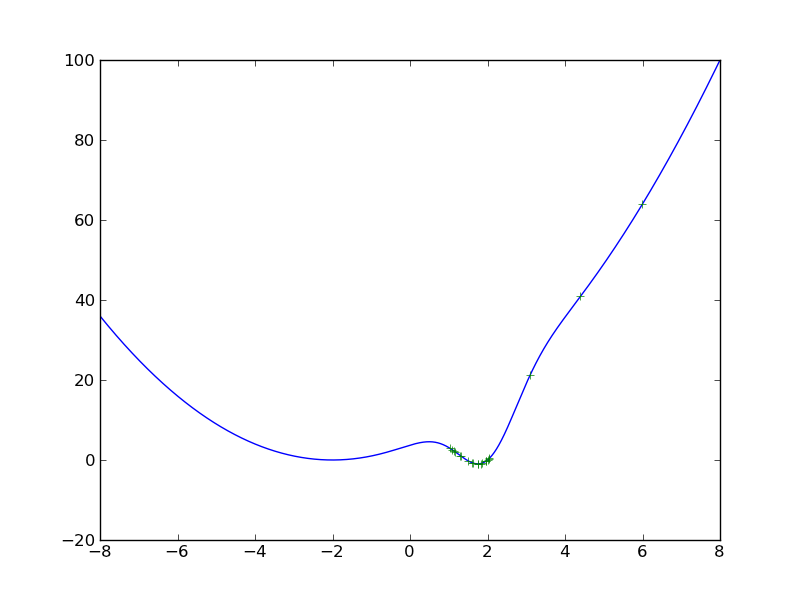
\includegraphics[width=1\columnwidth]{figs/intro/gradex2.png}
 \caption{\label{fig:gradex2} Example of running gradient descent
   starting on point $x_0 = 8$ for function $f(x) = (x+2)^2 - 16
   \exp\left( -(x-2)^2 \right)$. The function is represented in blue,
   while the points of the minimizing sequence are displayed as green
   pluses.}
\end{center}
\end{figure}


Figure \ref{fig:gradex2} shows the resulting minimizing sequence. Note
that now the algorithm converged to the global minimum. However, note
that to get to the global minimum the sequence of points jumped from one side of the minimum to the other. This is a consequence of using a wrong step size (in this case too large).


Repeat the previous exercise changing both the values of the step-size and the precision. What do you observe?
\end{exercise}

During this school we will rely on the numerical optimization methods provided by Scipy (scientific computing library in python), which are very efficient implementations.


% \begin{exercise}
% Consider the linear regression problem (ordinary least squares), with a
% single response variable

% \[
% y = x^T w + \varepsilon
% \]

% The \emph{linear regression problem} is, given a set $\{ y^{(i)} \}_i$ of
% samples of $y$ and the corresponding $\vect{x}^{(i)}$ vectors, estimate
% $\vect{w}$ to minimise the sum of the $\varepsilon$ variables. Traditionally
% this is solved analytically to obtain a closed form solution (although this is
% \textbf{not the way in which it should be computed}, linear algebra packages
% have an optimised solver, with numpy, use \code{numpy.linalg.lstsq}).

% Alternatively, we can define the error function for each possible $\vect{w}$:

% \[
% e(\vect{w}) = \sum_i \left( {\vect{x}^{(i)}}^T \vect{w} - y^{(i)} \right)^2.
% \]

% \begin{enumerate}
% \item Derive the gradient of the error $\pd{e}{w_j}$.
% \item Implement a solver based on this for two dimensional problems (i.e.,
% $\vect{w} \in R^2$).
% \item Use this method on the Galton dataset from the previous exercise to
% estimate the relationship between father and son's height. Try two formulas
% \begin{equation}
% s = f w_1 + \varepsilon,
% \label{}
% \end{equation}
% where $s$ is the son's height, and $f$ is the father heights; and
% \begin{equation}
% s = f w_1 + 1w_0 + \varepsilon
% \label{}
% \end{equation}
% where the input variable is now two dimensional: $(f,1)$. This allows the
% intercept to be non-zero.
% \item Plot the regression line you obtain with the points from the previous
% exercise.
% \item Use the \texttt{np.linalg.lstsq} function and compare to your solution.
% \end{enumerate}
% \end{exercise}



%Basic concepts of numerical optimization.

%\begin{itemize}
%\item - Gradient base methods, gradient descent, its problems,
%  conjugate and lbfgs. Can use routines from python, make example with
%  Gaussian with different variates and show the behavior.
%\item convex functions vs non convex functions, very brief, convex
%  function is like a bowl, if you drop a ball from the top it will
%  reach the bottom, Non-convex several bottom, will reach one of them.
%\item Gradient, sub-gradient generalization
%\end{itemize}


% \subsection{Matrix Derivatives}

% In subsection we finalize by showing some basic formulas for the
% gradient of matrix:

% \begin{itemize}
% \item For vectors $a$ and $x$, $\frac{\partial a^{T} x}{\partial x}= a$
% \item For vectors $a$ and $x$ and matrix $A$, $\frac{\partial a^{T}Ab}{\partial A} = ab^{T}$
% \item For vectors $a$ and $x$ and matrix $A$, $\frac{\partial a^{T}A^{T}b}{\partial A} =  ba^{T}$
% \end{itemize}

% {\bf The Gradient: }Suppose that $f:\mathbb{R}^{m\times n} \rightarrow\mathbb{R}$ is a function that takes as input, a matrix $A$
% of size $m\times n$ and returns a real value. Then the {\bf gradient} of $f$ (with respect to $A\in \mathbb{R}^{m\times n}$)
% is the matrix of partial derivatives, defined as:
% \begin{equation*}
% \nabla_{A}f(A)\in \mathbb{R}^{m\times n} = \left[\begin{array}{cccc}
% \frac{\partial f(A)}{\partial A_{11}} & \frac{\partial f(A)}{\partial A_{12}} & \ldots & \frac{\partial f(A)}{\partial A_{1n}} \\
% \frac{\partial f(A)}{\partial A_{21}} & \frac{\partial f(A)}{\partial A_{22}} & \ldots & \frac{\partial f(A)}{\partial A_{2n}} \\
% \vdots & \vdots &\ddots & \vdots \\
% \frac{\partial f(A)}{\partial A_{m1}} & \frac{\partial f(A)}{\partial A_{m2}} & \ldots & \frac{\partial f(A)}{\partial A_{mn}} \\
% \end{array}\right].
% \end{equation*}

% The gradient is defined {\em only} if the function is real-valued, that is, if it returns a scalar value. Some 
% important properties:

% \begin{itemize}
% \item $\nabla_{x}(f(x) + g(x)) = \nabla_{x}f(x) + \nabla_{x}g(x)$.
% \item For $t \in \mathbb{R}$, $\nabla_{x}(tf(x))= t\nabla_{x}f(x)$.
% \item Let $f:\mathbb{R}^{m} \rightarrow \mathbb{R}$ be the function defined by $f(z)=z^{T}z$, $\nabla_{z}f(z)=2z$.
% \end{itemize}
% {\bf The Hessian:} Suppose that $f:\mathbb{R}^{n}\rightarrow\mathbb{R}$ is a function that takes a vector in $\mathbb{R}^{n}$ and
% returns a real number, then the {\em Hessian} matrix with respect to $x$, written $\nabla_{x}^{2}f(x)$ (or $H$) is the $n\times n$
% matrix of partial derivatives,

% \begin{equation*}
% \nabla_{x}^{2}f(x) \in \mathbb{R}^{n\times n}= \left[\begin{array}{cccc}
% \frac{\partial^{2}f(x)}{\partial x_{1}^{2}} & \frac{\partial^{2}f(x)}{\partial x_{1} \partial x_{2}} & \ldots &  \frac{\partial^{2}f(x)}{\partial x_{1} \partial x_{n}} \\
% \frac{\partial^{2}f(x)}{\partial x_{2} \partial x_{1}} & \frac{\partial^{2}f(x)}{\partial x_{2}^{2}} & \ldots &  \frac{\partial^{2}f(x)}{\partial x_{2} \partial x_{n}} \\
% \vdots & \vdots & \ddots & \vdots \\
% \frac{\partial^{2}f(x)}{\partial x_{n} \partial x_{1}} & \frac{\partial^{2}f(x)}{\partial x_{n}\partial x_{2}} & \ldots &  \frac{\partial^{2}f(x)}{\partial x_{n}^{2}} 

% \end{array}\right].
% \end{equation*}

% Note that the Hessian is always symmetric, since
% \begin{equation*}
% \frac{\partial^{2}f(x)}{\partial x_{i}\partial x_{j}} =\frac{\partial^{2}f(x)}{\partial x_{j}\partial x_{i}}.
% \end{equation*}



%%% Local Variables: 
%%% mode: latex
%%% TeX-master: "../../guide"
%%% End: 
